\documentclass[letterpaper,12pt]{article}\usepackage[]{graphicx}\usepackage[]{color}
%% maxwidth is the original width if it is less than linewidth
%% otherwise use linewidth (to make sure the graphics do not exceed the margin)
\makeatletter
\def\maxwidth{ %
  \ifdim\Gin@nat@width>\linewidth
    \linewidth
  \else
    \Gin@nat@width
  \fi
}
\makeatother

\definecolor{fgcolor}{rgb}{0.345, 0.345, 0.345}
\newcommand{\hlnum}[1]{\textcolor[rgb]{0.686,0.059,0.569}{#1}}%
\newcommand{\hlstr}[1]{\textcolor[rgb]{0.192,0.494,0.8}{#1}}%
\newcommand{\hlcom}[1]{\textcolor[rgb]{0.678,0.584,0.686}{\textit{#1}}}%
\newcommand{\hlopt}[1]{\textcolor[rgb]{0,0,0}{#1}}%
\newcommand{\hlstd}[1]{\textcolor[rgb]{0.345,0.345,0.345}{#1}}%
\newcommand{\hlkwa}[1]{\textcolor[rgb]{0.161,0.373,0.58}{\textbf{#1}}}%
\newcommand{\hlkwb}[1]{\textcolor[rgb]{0.69,0.353,0.396}{#1}}%
\newcommand{\hlkwc}[1]{\textcolor[rgb]{0.333,0.667,0.333}{#1}}%
\newcommand{\hlkwd}[1]{\textcolor[rgb]{0.737,0.353,0.396}{\textbf{#1}}}%
\let\hlipl\hlkwb

\usepackage{framed}
\makeatletter
\newenvironment{kframe}{%
 \def\at@end@of@kframe{}%
 \ifinner\ifhmode%
  \def\at@end@of@kframe{\end{minipage}}%
  \begin{minipage}{\columnwidth}%
 \fi\fi%
 \def\FrameCommand##1{\hskip\@totalleftmargin \hskip-\fboxsep
 \colorbox{shadecolor}{##1}\hskip-\fboxsep
     % There is no \\@totalrightmargin, so:
     \hskip-\linewidth \hskip-\@totalleftmargin \hskip\columnwidth}%
 \MakeFramed {\advance\hsize-\width
   \@totalleftmargin\z@ \linewidth\hsize
   \@setminipage}}%
 {\par\unskip\endMakeFramed%
 \at@end@of@kframe}
\makeatother

\definecolor{shadecolor}{rgb}{.97, .97, .97}
\definecolor{messagecolor}{rgb}{0, 0, 0}
\definecolor{warningcolor}{rgb}{1, 0, 1}
\definecolor{errorcolor}{rgb}{1, 0, 0}
\newenvironment{knitrout}{}{} % an empty environment to be redefined in TeX

\usepackage{alltt}
\usepackage[top=1in,bottom=1in,left=1in,right=1in]{geometry}
\usepackage{setspace}
\usepackage[colorlinks=true,urlcolor=blue,citecolor=blue,linkcolor=blue]{hyperref}
\usepackage{indentfirst}
\usepackage{multirow}
\usepackage{booktabs}
\usepackage[final]{animate}
\usepackage{graphicx}
\usepackage{verbatim}
\usepackage{rotating}
\usepackage{tabularx}
\usepackage{array}
\usepackage{subfig} 
\usepackage[noae]{Sweave}
\usepackage{cleveref}
\usepackage[figureposition=bottom]{caption}
\usepackage{paralist}
\usepackage{acronym}
\usepackage{outlines}
\usepackage{pdflscape}

% housekeeping


\linespread{1}
\IfFileExists{upquote.sty}{\usepackage{upquote}}{}
\begin{document}
\title{Analysis of crab abundance, presence/absence, and carapace length}
\maketitle

\section{Regression}



\begin{knitrout}
\definecolor{shadecolor}{rgb}{0.969, 0.969, 0.969}\color{fgcolor}
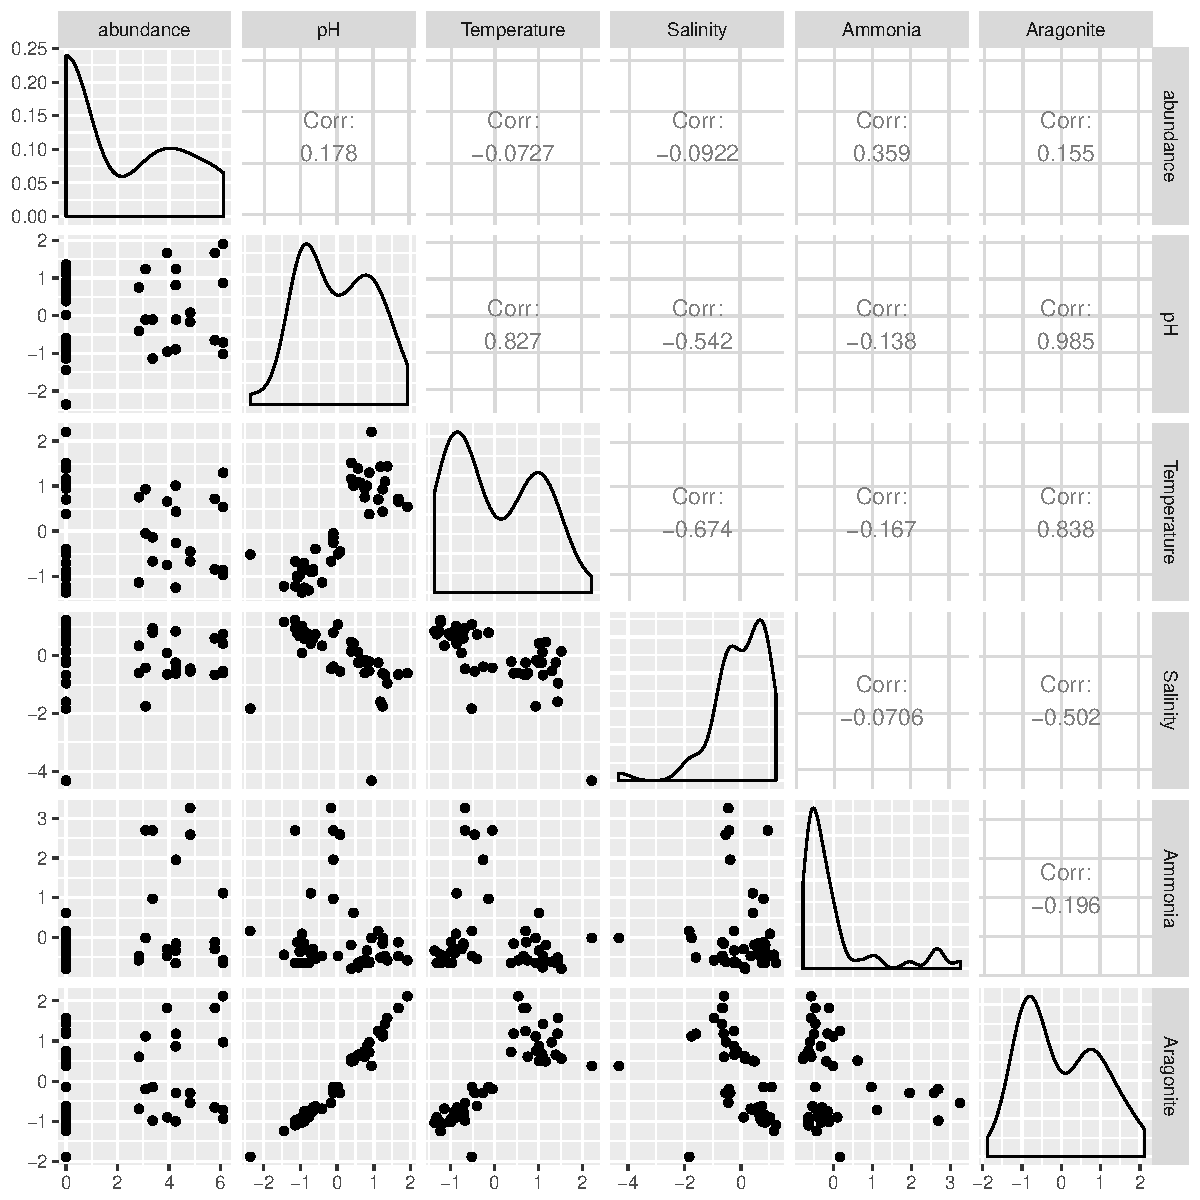
\includegraphics[width=0.8\textwidth]{figure/unnamed-chunk-3-1} 

\end{knitrout}



\begin{knitrout}
\definecolor{shadecolor}{rgb}{0.969, 0.969, 0.969}\color{fgcolor}\begin{figure}
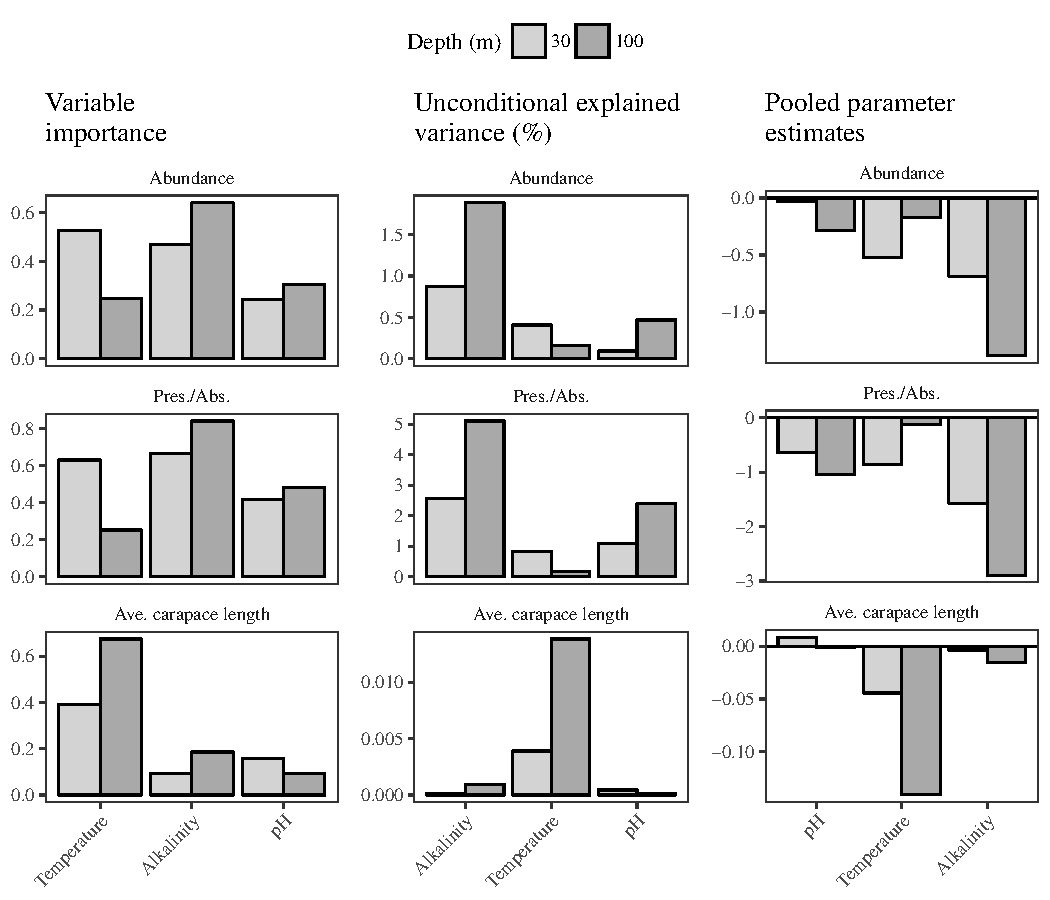
\includegraphics[width=\maxwidth]{figure/unnamed-chunk-5-1} \caption[Results of model selection analysis with three crab population variables (abundance, presence/absence, carapace length) by shallow and deep water]{Results of model selection analysis with three crab population variables (abundance, presence/absence, carapace length) by shallow and deep water. Variable importances and pooled estimates show summarized results from multiple models that evaluated all parameter combinations.  The unconditional explained variance (\%) is the effect of each variable independent of all other variables.}\label{fig:unnamed-chunk-5}
\end{figure}


\end{knitrout}
\clearpage

\begin{landscape}
\centering\vspace*{\fill}
%latex.default(abutab[, -c(1, 2)], file = "", rowlabel = "Models",     caption = cap.val, caption.loc = "top", rgroup = unique(abutab$depth),     n.rgroup = c(5, 5), rowname = abutab$model, size = "scriptsize",     label = "tab:abutab")%
\begin{table}[!tbp]
{\scriptsize
\caption{Top five selected models for crab abundance at shallow and deep water. Input variables were aragonite, fluorescence, nitrate, oxygen, ph, and salinity. All explanatory variables were scaled and centered.\label{tab:abutab}} 
\begin{center}
\begin{tabular}{llllllllllll}
\hline\hline
\multicolumn{1}{l}{Models}&\multicolumn{1}{c}{Int.}&\multicolumn{1}{c}{Aragonite}&\multicolumn{1}{c}{Fluorescence}&\multicolumn{1}{c}{Nitrate}&\multicolumn{1}{c}{Oxygen}&\multicolumn{1}{c}{pH}&\multicolumn{1}{c}{Salinity}&\multicolumn{1}{c}{df}&\multicolumn{1}{c}{logLik}&\multicolumn{1}{c}{AICc}&\multicolumn{1}{c}{delta}\tabularnewline
\hline
{\bfseries 30 m}&&&&&&&&&&&\tabularnewline
~~1&2.68&-&-&1.49&-&-&-2.17&4&-47.51&105.24&0\tabularnewline
~~2&1.43&-&0.87&-&-&-&-1.88&4&-47.6&105.43&0.19\tabularnewline
~~3&1.96&-&0.74&-&-&-0.79&-2.36&5&-47.03&107.58&2.34\tabularnewline
~~4&2.13&-&0.48&0.89&-&-&-2.12&5&-47.04&107.61&2.37\tabularnewline
~~5&1.78&-&0.86&-&-0.57&-&-2.29&5&-47.22&107.96&2.72\tabularnewline
\hline
{\bfseries 100 m}&&&&&&&&&&&\tabularnewline
~~1&3.16&-&1.29&-&-&-&-1.99&4&-47.66&105.54&0\tabularnewline
~~2&2.75&-&-&-&-&-&-1.85&3&-49.78&106.83&1.29\tabularnewline
~~3&3.11&-&1.53&-&7.28&-7.44&-&5&-46.78&107.09&1.55\tabularnewline
~~4&2.52&-&-&-&-&-1.25&-2.81&4&-48.86&107.94&2.4\tabularnewline
~~5&2.31&-1.28&-&-&-&-&-2.53&4&-49.02&108.26&2.72\tabularnewline
\hline
\end{tabular}\end{center}}
\end{table}
%latex.default(patab[, -c(1, 2)], file = "", rowlabel = "Models",     caption = cap.val, caption.loc = "top", rgroup = unique(patab$depth),     n.rgroup = c(5, 5), rowname = patab$model, size = "scriptsize",     label = "tab:patab")%
\begin{table}[!tbp]
{\scriptsize
\caption{Top five selected models for crab presence/absence at shallow and deep water. Input variables were aragonite, fluorescence, nitrate, oxygen, ph, and salinity. All explanatory variables were scaled and centered.\label{tab:patab}} 
\begin{center}
\begin{tabular}{llllllllllll}
\hline\hline
\multicolumn{1}{l}{Models}&\multicolumn{1}{c}{Int.}&\multicolumn{1}{c}{Aragonite}&\multicolumn{1}{c}{Fluorescence}&\multicolumn{1}{c}{Nitrate}&\multicolumn{1}{c}{Oxygen}&\multicolumn{1}{c}{pH}&\multicolumn{1}{c}{Salinity}&\multicolumn{1}{c}{df}&\multicolumn{1}{c}{logLik}&\multicolumn{1}{c}{AICc}&\multicolumn{1}{c}{delta}\tabularnewline
\hline
{\bfseries 30}&&&&&&&&&&&\tabularnewline
~~1&1.17&-&-&2.62&-&-&-3.15&3&-10.22&27.71&0\tabularnewline
~~2&1.08&-&-&-&-&-2.79&-4.17&3&-10.51&28.28&0.57\tabularnewline
~~3&1&-2.27&-&-&-&-&-3.29&3&-11.07&29.39&1.69\tabularnewline
~~4&0.49&-&0.81&-&-&-2.27&-4.08&4&-9.61&29.44&1.73\tabularnewline
~~5&-0.07&-&1.17&-&-1.95&-&-4.1&4&-9.71&29.65&1.94\tabularnewline
\hline
{\bfseries 100}&&&&&&&&&&&\tabularnewline
~~1&3.34&-&3.41&-&-&-&-5.46&3&-7.53&22.33&0\tabularnewline
~~2&3.31&-&3.27&0.37&-&-&-5.85&4&-7.5&25.22&2.89\tabularnewline
~~3&3.29&-&3.24&-&-&-0.42&-5.84&4&-7.51&25.24&2.91\tabularnewline
~~4&3.24&-0.28&3.3&-&-&-&-5.62&4&-7.53&25.27&2.94\tabularnewline
~~5&3.34&-&3.34&-&-0.2&-&-5.72&4&-7.53&25.28&2.94\tabularnewline
\hline
\end{tabular}\end{center}}
\end{table}

\end{landscape}

\begin{landscape}
\centering\vspace*{\fill}
%latex.default(cltab[, -c(1, 2)], file = "", rowlabel = "Models",     caption = cap.val, caption.loc = "top", rgroup = unique(cltab$depth),     n.rgroup = c(5, 5), rowname = cltab$model, size = "scriptsize",     label = "tab:cltab")%
\begin{table}[!tbp]
{\scriptsize
\caption{Top five selected models for crab carapace length at shallow and deep water. Input variables were aragonite, fluorescence, nitrate, oxygen, ph, and salinity.  All explanatory variables were scaled and centered.\label{tab:cltab}} 
\begin{center}
\begin{tabular}{llllllllllll}
\hline\hline
\multicolumn{1}{l}{Models}&\multicolumn{1}{c}{Int.}&\multicolumn{1}{c}{Aragonite}&\multicolumn{1}{c}{Fluorescence}&\multicolumn{1}{c}{Nitrate}&\multicolumn{1}{c}{Oxygen}&\multicolumn{1}{c}{pH}&\multicolumn{1}{c}{Salinity}&\multicolumn{1}{c}{df}&\multicolumn{1}{c}{logLik}&\multicolumn{1}{c}{AICc}&\multicolumn{1}{c}{delta}\tabularnewline
\hline
{\bfseries 30}&&&&&&&&&&&\tabularnewline
~~1&6.59&-&-&-&-&-&-&2&6.99&-8.28&0\tabularnewline
~~2&6.61&-&-&0.06&-&-&-&3&7.7&-5.41&2.87\tabularnewline
~~3&6.6&-0.03&-&-&-&-&-&3&7.34&-4.68&3.6\tabularnewline
~~4&6.6&-&-&-&-&-0.02&-&3&7.12&-4.23&4.04\tabularnewline
~~5&6.57&-&0.01&-&-&-&-&3&7.11&-4.21&4.06\tabularnewline
\hline
{\bfseries 100}&&&&&&&&&&&\tabularnewline
~~1&6.59&-&-&-&-&-&-&2&6.99&-8.28&0\tabularnewline
~~2&6.42&-0.63&-&-&-&0.41&-&4&12.07&-8.14&0.13\tabularnewline
~~3&6.54&-&-&0.1&-&-&-&3&8.33&-6.66&1.61\tabularnewline
~~4&6.46&-0.42&-&-&0.23&-&-&4&11.25&-6.5&1.78\tabularnewline
~~5&6.52&-0.11&-&-&-&-&-&3&8.21&-6.41&1.86\tabularnewline
\hline
\end{tabular}\end{center}}
\end{table}

\end{landscape}

\section{PCA regression}

\begin{knitrout}
\definecolor{shadecolor}{rgb}{0.969, 0.969, 0.969}\color{fgcolor}\begin{figure}[!h]
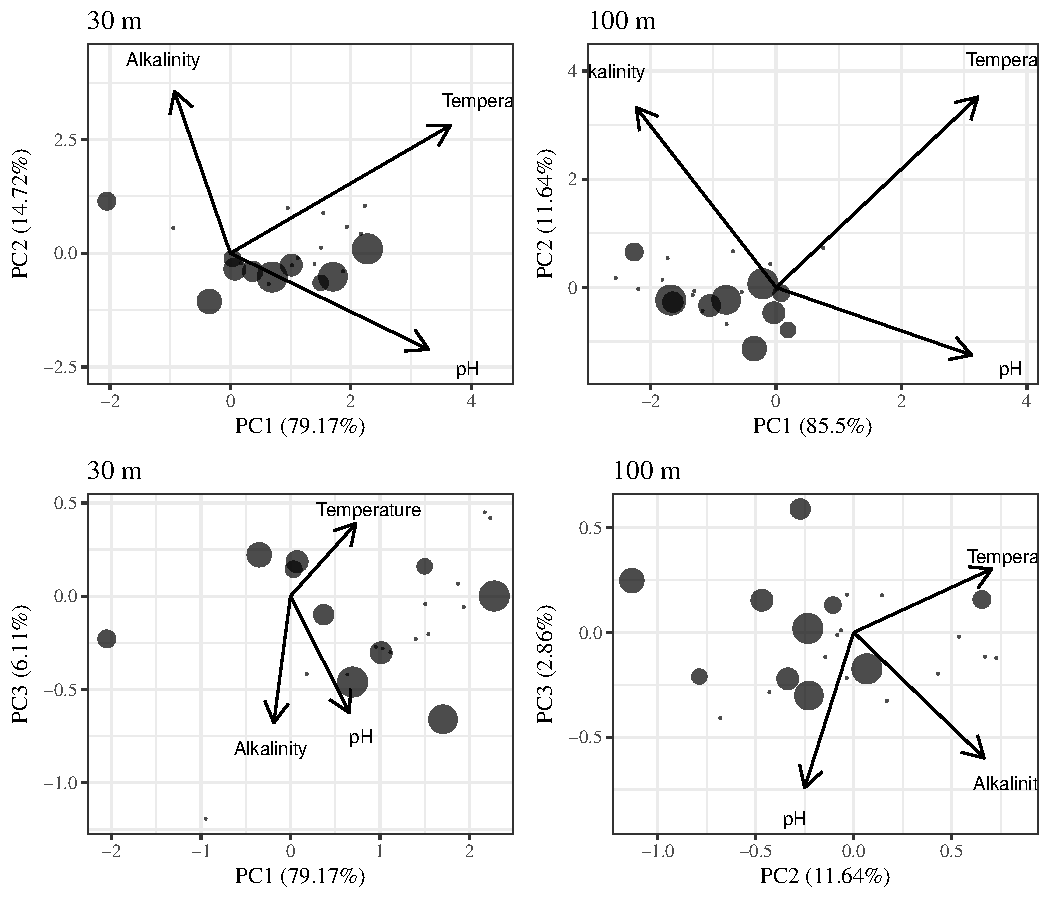
\includegraphics[width=0.9\textwidth]{figure/unnamed-chunk-8-1} \caption[PCA results, points sized by abundance]{PCA results, points sized by abundance}\label{fig:unnamed-chunk-8}
\end{figure}


\end{knitrout}



\begin{knitrout}
\definecolor{shadecolor}{rgb}{0.969, 0.969, 0.969}\color{fgcolor}\begin{figure}
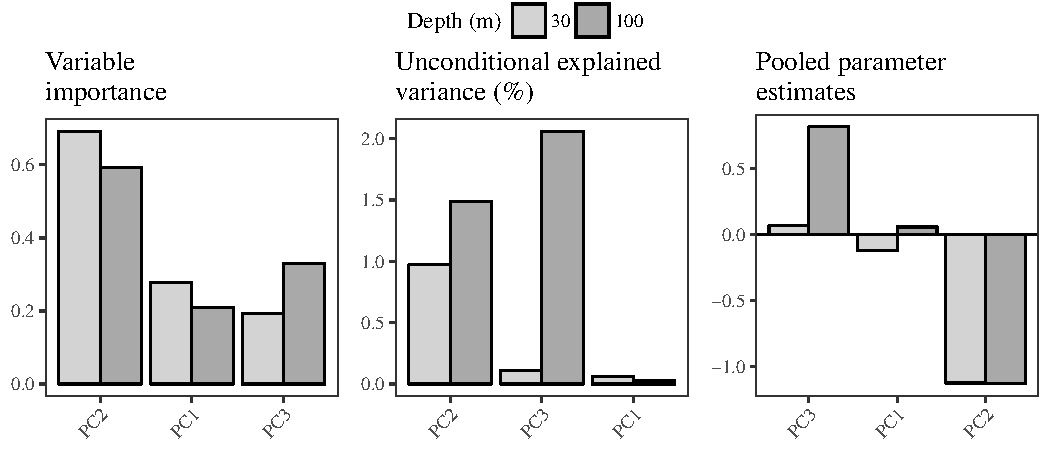
\includegraphics[width=\maxwidth]{figure/unnamed-chunk-10-1} \caption[Results of model selection analysis with crab abundance, by shallow and deep water]{Results of model selection analysis with crab abundance, by shallow and deep water. Models were created using four principal components of input variables. Importances and pooled estimates show summarized results from multiple models that evaluated all parameter combinations.  The unconditional explained variance (\%) is the effect of each axis independent of all other variables.}\label{fig:unnamed-chunk-10}
\end{figure}


\end{knitrout}

\begin{landscape}
\centering\vspace*{\fill}
%latex.default(abutab[, -c(1, 2)], file = "", rowlabel = "Models",     caption = cap.val, caption.loc = "top", rgroup = unique(abutab$depth),     n.rgroup = c(5, 5), rowname = abutab$model, size = "scriptsize",     label = "tab:abutabpca")%
\begin{table}[!tbp]
{\scriptsize
\caption{Top five selected models for crab abundance at shallow and deep water using principal component axes. Input variables for PCA were aragonite, fluorescence, nitrate, oxygen, ph, and salinity. All explanatory variables were scaled and centered.\label{tab:abutabpca}} 
\begin{center}
\begin{tabular}{llllllllll}
\hline\hline
\multicolumn{1}{l}{Models}&\multicolumn{1}{c}{Int.}&\multicolumn{1}{c}{PC1}&\multicolumn{1}{c}{PC2}&\multicolumn{1}{c}{PC3}&\multicolumn{1}{c}{PC4}&\multicolumn{1}{c}{df}&\multicolumn{1}{c}{logLik}&\multicolumn{1}{c}{AICc}&\multicolumn{1}{c}{delta}\tabularnewline
\hline
{\bfseries 30 m}&&&&&&&&&\tabularnewline
~~1&1.92&-&-0.63&-2.03&-&4&-47.44&105.1&0\tabularnewline
~~2&2.23&-&-&-2.17&-&3&-49.02&105.31&0.21\tabularnewline
~~3&2.74&-0.35&-&-2.4&-&4&-48.32&106.86&1.76\tabularnewline
~~4&1.83&-&-0.66&-1.99&1.04&5&-47.15&107.83&2.74\tabularnewline
~~5&2.17&-&-&-2.14&0.77&4&-48.89&108&2.9\tabularnewline
\hline
{\bfseries 100 m}&&&&&&&&&\tabularnewline
~~1&2.23&-&-1.22&2.03&-&4&-48.8&107.82&0\tabularnewline
~~2&3.19&0.62&-1.72&-&-&4&-48.95&108.12&0.3\tabularnewline
~~3&3.06&0.57&-1.65&1.89&-&5&-47.3&108.14&0.32\tabularnewline
~~4&2.29&-&-1.26&-&-&3&-50.49&108.24&0.42\tabularnewline
~~5&1.88&-&-&2.1&-&3&-50.63&108.52&0.7\tabularnewline
\hline
\end{tabular}\end{center}}
\end{table}

\end{landscape}

\begin{landscape}
\centering\vspace*{\fill}
%latex.default(tab[, -c(1, 2)], file = "", rowlabel = "Models",     caption = cap.val, caption.loc = "top", rgroup = unique(tab$depth),     n.rgroup = table(tab$depth), rowname = tab$dt, label = "tab:pcacor")%
\begin{table}[!tbp]
\caption{Correlations of crab abundance and input variables with principal component (PC) axes. Abundance was modelled with PC axes created using the input variables.\label{tab:pcacor}} 
\begin{center}
\begin{tabular}{lllll}
\hline\hline
\multicolumn{1}{l}{Models}&\multicolumn{1}{c}{PC1}&\multicolumn{1}{c}{PC2}&\multicolumn{1}{c}{PC3}&\multicolumn{1}{c}{PC4}\tabularnewline
\hline
{\bfseries 30 m}&&&&\tabularnewline
~~Abundance&-0.09&-0.36&-0.49*&0.12\tabularnewline
~~Aragonite&0.96*&0.24&-0.11&-0.19\tabularnewline
~~Fluorescence&-0.52*&-0.98*&-0.03&0\tabularnewline
~~Nitrate&-0.89*&-0.65*&-0.03&-0.01\tabularnewline
~~Oxygen&0.87*&-0.03&-0.39&-0.5*\tabularnewline
~~pH&0.98*&0.23&-0.28&-0.27\tabularnewline
~~Salinity&-0.56*&-0.11&0.91*&-0.17\tabularnewline
\hline
{\bfseries 100 m}&&&&\tabularnewline
~~Abundance&0.16&-0.37&0.35&0.04\tabularnewline
~~Aragonite&0.95*&0.42*&-0.13&0.08\tabularnewline
~~Fluorescence&-0.39&-0.99*&-0.08&0.03\tabularnewline
~~Nitrate&-0.94*&-0.36&0.19&-0.37\tabularnewline
~~Oxygen&0.98*&0.41*&0.13&0\tabularnewline
~~pH&0.99*&0.44*&0.03&0.02\tabularnewline
~~Salinity&-0.73*&-0.01&-0.65*&-0.28\tabularnewline
\hline
\end{tabular}\end{center}
\end{table}

\end{landscape}

\end{document}
